\chapter{What you did}
\label{ch:whatYouDid}


% \engExpl{Choose your own chapter title to describe this}
% \sweExpl{[Vad gjorde du? Hur gick det till? – Välj lämplig rubrik (“Genomförande”, “Konstruktion”, ”Utveckling”  eller annat]}


% \engExpl{What have you done? How did you do it? What design decisions did you make? How did what you did help you to meet your goals?}
% \sweExpl{Vad du har gjort? Hur gjorde du det? Vilka designval gjorde du?\\
% Hur kom det du hjälpte dig att uppnå dina mål?}


% the following sets the TOC entry to break after the & - note you have to include the first letter of the following word as it get swolled by the \texorpdfstring{}{} processing


% \section[Hardware/Software design …/Model/Simulation model \&\texorpdfstring{\\}{ p} parameters/…]{Hardware/Software design …/Model/Simulation model \& parameters/…}


\section{Proof of Concepts}


The following section will outline the various \gls{POC} applications that were built before the actual software that was written to conduct the research outlined in this thesis. Each \gls{POC} will outline what it was trying to accomplish and what the outcome was.


\subsection{Langchain based applications}


Langchain is a company \footnote{\href{https://langchain.com}{langchain.com}} and framework \footnote{\href{https://python.langchain.com}{python.langchain.com}} for building context aware reasoning applications. The framework allows for easy composition of language models and \gls{RAG} techniques and tools that makes it easy to build chatbots with a connected knowledge base. This section outlines some \gls{POC}s that were made with the langchain framework.


\subsubsection{GPT-4 and text-embedding-3-large}
\label{sec:poc_gpt_langchain}


To build a chat application with an AI-assistant that has access to an external knowledge base, one of the most popular approaches is to use langchain to connect the following four parts.


\begin{enumerate}
        \item A \gls{LLM}, such as GPT-4 to run the chat.
        \item A \gls{LLM}, such as GPT-4 to run the query construction.
        \item An embedding function, such as OpenAI’s text-embedding-3-large used to index and query documents.
        \item A vector store, such as ChromaDB, that stores the vector embeddings and associated documents \footnote{\href{https://www.trychroma.com/}{trychroma.com/}}
\end{enumerate}.


In this configuration, Lanchain acts as the glue connecting these components and handling tasks like chunking larger documents. The goal of this \gls{POC} was to test a common approach for building AI assistants and evaluate its potential for use in the full study. \href{https://www.youtube.com/watch?v=bKjxi-NKRHo}{A video can be seen here} that showcases this \gls{POC}.


\subsubsection{Mistral 7B v0.2 and e5-large-v2}


There was a \gls{POC} constructed that had the same approach as the one outlined in \ref{sec:poc_gpt_langchain} with the notable requirement that all tools had to be under an open source licence. This meant the GPT-4 model and text-embedding-3-large models couldn’t be used. A similar version of the same \gls{POC} was made that used the Mistral 7B v0.2 model and the embedding function e5-large-v2 \cite{wang_text_2024}. These are both under an open source licence and are freely available on Huggingface \footnote{\href{https://huggingface.co/mistralai/Mistral-7B-Instruct-v0.2}{huggingface.co/mistralai/Mistral-7B-Instruct-v0.2} \href{https://huggingface.co/intfloat/e5-large-v2}{huggingface.co/intfloat/e5-large-v2}}. This \gls{POC} did however suffer from poor performance in initial tests for retrieval and performance. It was difficult to tune the prompts to get decent performance. This \gls{POC} showed it was difficult for the researcher to get good performance out of certain models using the langchain framework.


\subsection{Custom applications}


This section outlines some major and minor \gls{POC}s that were made without any frameworks that are popular \gls{LLM} applications, aside from very common python libraries such as pytorch and hugginface’s transformers library.


\subsubsection{Simple Python API for models on Huggingface}


Langchain and similar tools support running language models locally. However, working with the prompt templates in less advanced models than GPT-4 and achieving good retrieval and chat performance was challenging. Therefore, a simple \gls{POC} was developed to create higher-level Python abstraction APIs on top of the Hugging Face Transformers library that could be integrated into completely custom solutions. These APIs include examples like those shown in listings ~\ref{fig:python-apis-for-llm} and ~\ref{fig:python-apis-for-embeddings}. A short video \href{https://www.youtube.com/watch?v=VG16oWK_LUQ}{can be seen here} that demonstrates a chat application (without an integrated knowledge base) built on-top of these simple APIs.


\begin{listing}[H]
\centering
\renewcommand{\theFancyVerbLine}{\scriptsize\arabic{FancyVerbLine}}
\scriptsize
\begin{minted}[
frame=lines,
framesep=2mm,
baselinestretch=1.2,
fontsize=\scriptsize,
linenos
]{python}
def load_hf_model(
    model_path: str,
    device: str
) -> (transformers.AutoModelForCausalLM, transformers.AutoTokenizer):
    """
    Loads a Hugging Face causal language model and its tokenizer for a given
    model path and device.
    """

def generate_text(
    model: transformers.AutoModelForCausalLM,
    tokenizer: transformers.AutoTokenizer,
    device: str,
    params: Params,
    prompt: str
) -> str:
    """
    Generates text from a prompt using the specified model, tokenizer, and
    generation parameters.
    """

async def generate_text_streaming(
    model: transformers.AutoModelForCausalLM,
    tokenizer: transformers.AutoTokenizer,
    device: str,
    params: Params,
    prompt: str
) -> AsyncGenerator[str, None]:
    """
    Asynchronously generates text from a prompt, yielding tokens incrementally.
    Useful for streaming responses.
    """

def _tokenise_inputs(
    tokeniser: transformers.AutoTokenizer,
    input_texts: list[str],
    max_length: int = 8192
) -> dict:
    """
    Tokenizes the input texts with padding and truncation.
    """

def should_stop_generating(
    output_token_ids: list,
    tokenizer: transformers.AutoTokenizer,
    params: Params,
    token_id: int
) -> bool:
    """
    Determines whether to stop generating text based on stop conditions.
    """
\end{minted}
\caption{High level API on-top of Huggingface's tranformers library that can be used for generating text using models available on Huggingface.}
\label{fig:python-apis-for-llm}
\end{listing}

\begin{listing}[H]
\centering
\renewcommand{\theFancyVerbLine}{\scriptsize\arabic{FancyVerbLine}}
\scriptsize
\begin{minted}[
frame=lines,
framesep=2mm,
baselinestretch=1.2,
fontsize=\scriptsize,
linenos
]{python}
def load_hf_embedding_model(
    model_path: str,
    device: str
) -> (torch.nn.Module, transformers.AutoTokenizer):
    """
    Loads a Hugging Face embedding model and its tokenizer for a given model
    path and device.
    """

async def compute_embedding(
    model: torch.nn.Module,
    tokeniser: transformers.AutoTokenizer,
    text: str
) -> List[float]:
    """
    Computes and returns the normalized embedding for a given text using the
    specified model and tokenizer.
    """

def _compute_model_embeddings(
    model: torch.nn.Module,
    tokenised_inputs: dict
) -> torch.Tensor:
    """
    Computes the model embeddings from the tokenized inputs.
    """
\end{minted}
\caption{High level API on-top of Huggingface's tranformers library that can be used for generating vector embeddings using models available on Huggingface.}
\label{fig:python-apis-for-embeddings}
\end{listing}



\subsubsection{Mistral 7B v0.2 and Opensearch}


The goal with this \gls{POC} was to build a version of the \gls{RAG} application that didn’t use a vector embedding function. Instead, this \gls{POC} would utilise a traditional search service such as Elasticsearch or Opensearch. These implement "traditional" search algorithms such as \gls{TF-IDF}, as outlined in section \ref{sec:background_tfidf}. This \gls{POC} was very easy to implement and showed great promise.


\subsubsection{Post processing for smaller models}


When working with models that don’t produce the best scores on public benchmarks, such as \gls{MMLU}, there are a number of techniques that can be employed that could improve the performance of a \gls{RAG} system. These generally smaller models suffer from worse scores on precision and recall benchmarks. This means they are worse at recalling facts injected into the conversation by a \gls{RAG} pipeline. One of the techniques that can be used is post-processing retrieved documents before they are inserted into the chat. There are a number of ways of achieving this. One of the techniques that was tried, and eventually implemented in the final study, was to use a post-processing mechanism, where each of the retrieved documents are passed through a post-processing function, which reduce the size of the document, as shown in \autoref{eq:without_post_processing} and \autoref{eq:with_post_processing}.


\begin{equation}
R = \text{LLM}\left(Q, \{D_i\}_{i=1}^N\right)
\label{eq:without_post_processing}
\end{equation}


Where:
\begin{itemize}
        \item \( R \) is the generated response.
        \item \( \text{LLM} \) is the language model function.
        \item \( Q \) is the user query.
        \item \( \{D_i\}_{i=1}^N \) are the matching documents retrieved from the index.
\end{itemize}


\begin{equation}
R = \text{LLM}\left(Q, \{\text{PP}(D_i, P)\}_{i=1}^N\right)
\label{eq:with_post_processing}
\end{equation}


Where:
\begin{itemize}
        \item \( \text{PP} \) is the post-processing function.
        \item \( P \) is the post-processing prompt.
\end{itemize}


There are different strategies for the prompt that reduce the size of the document. This prompt can instruct the language model to extract quotes from the document related to the query, summarise key facts related to the query, or a number of other methods. The one that was chosen for the final study was extracting quotes as this showed the most potential. \autoref{fig:without_post_processing} and \autoref{fig:with_post_processing} illustrate this process.


% https://lucid.app/lucidchart/7d7e52da-e0c5-45de-9d50-6fc1313b1528/edit

\begin{figure}[H]
    \centering
    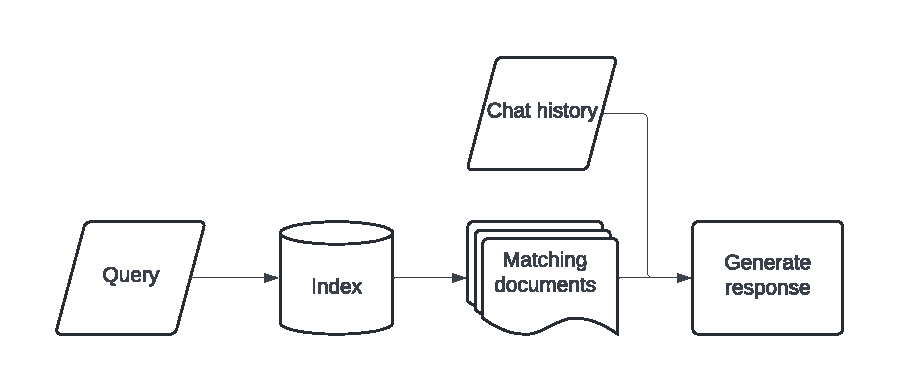
\includegraphics[width=\textwidth]{content/figures/assets/10-without-post-processing.pdf}
    \caption{Diagram that shows how documents are injected into the chat, without post-processing}
    \label{fig:without_post_processing}
\end{figure}



% https://lucid.app/lucidchart/f126e1c6-7c22-4445-8977-d2e8ccfba351/edit

\begin{figure}[H]
    \centering
    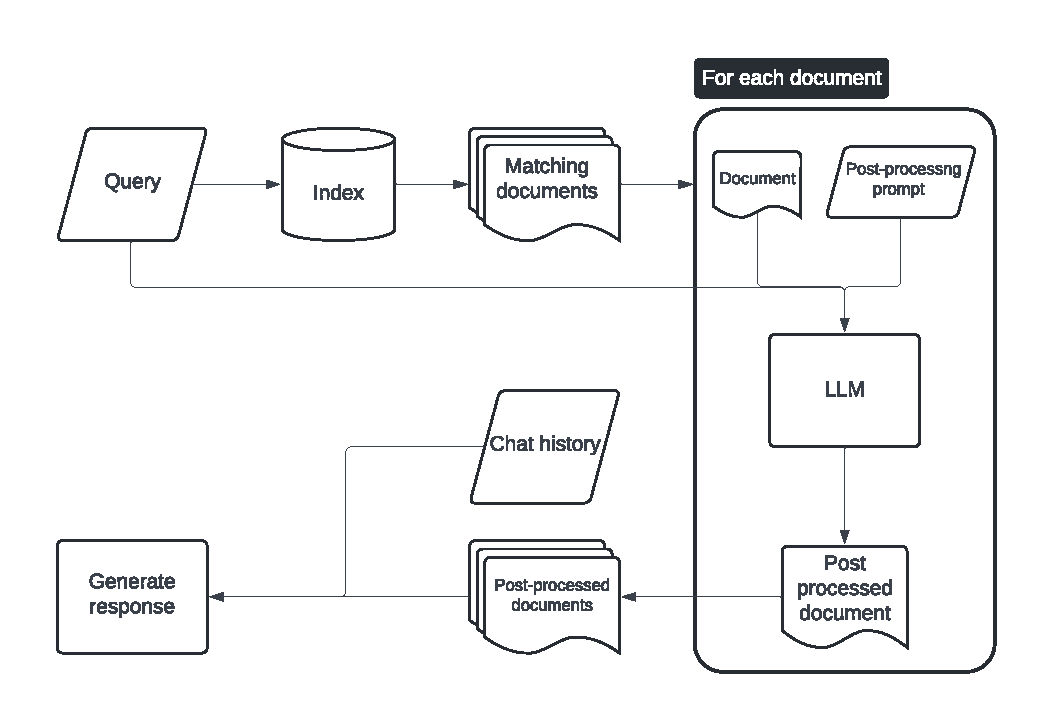
\includegraphics[width=\textwidth]{content/figures/assets/11-with-processing.pdf}
    \caption{Diagram that shows how documents are post-processed before they are injected into the chat}
    \label{fig:with_post_processing}
\end{figure}



\subsubsection{Too much post processing}


\section{The architecture of the software}


% https://lucid.app/lucidchart/f5dc4477-fa25-44e8-93d9-946def9cd4a9/edit

\begin{figure}[H]
    \centering
    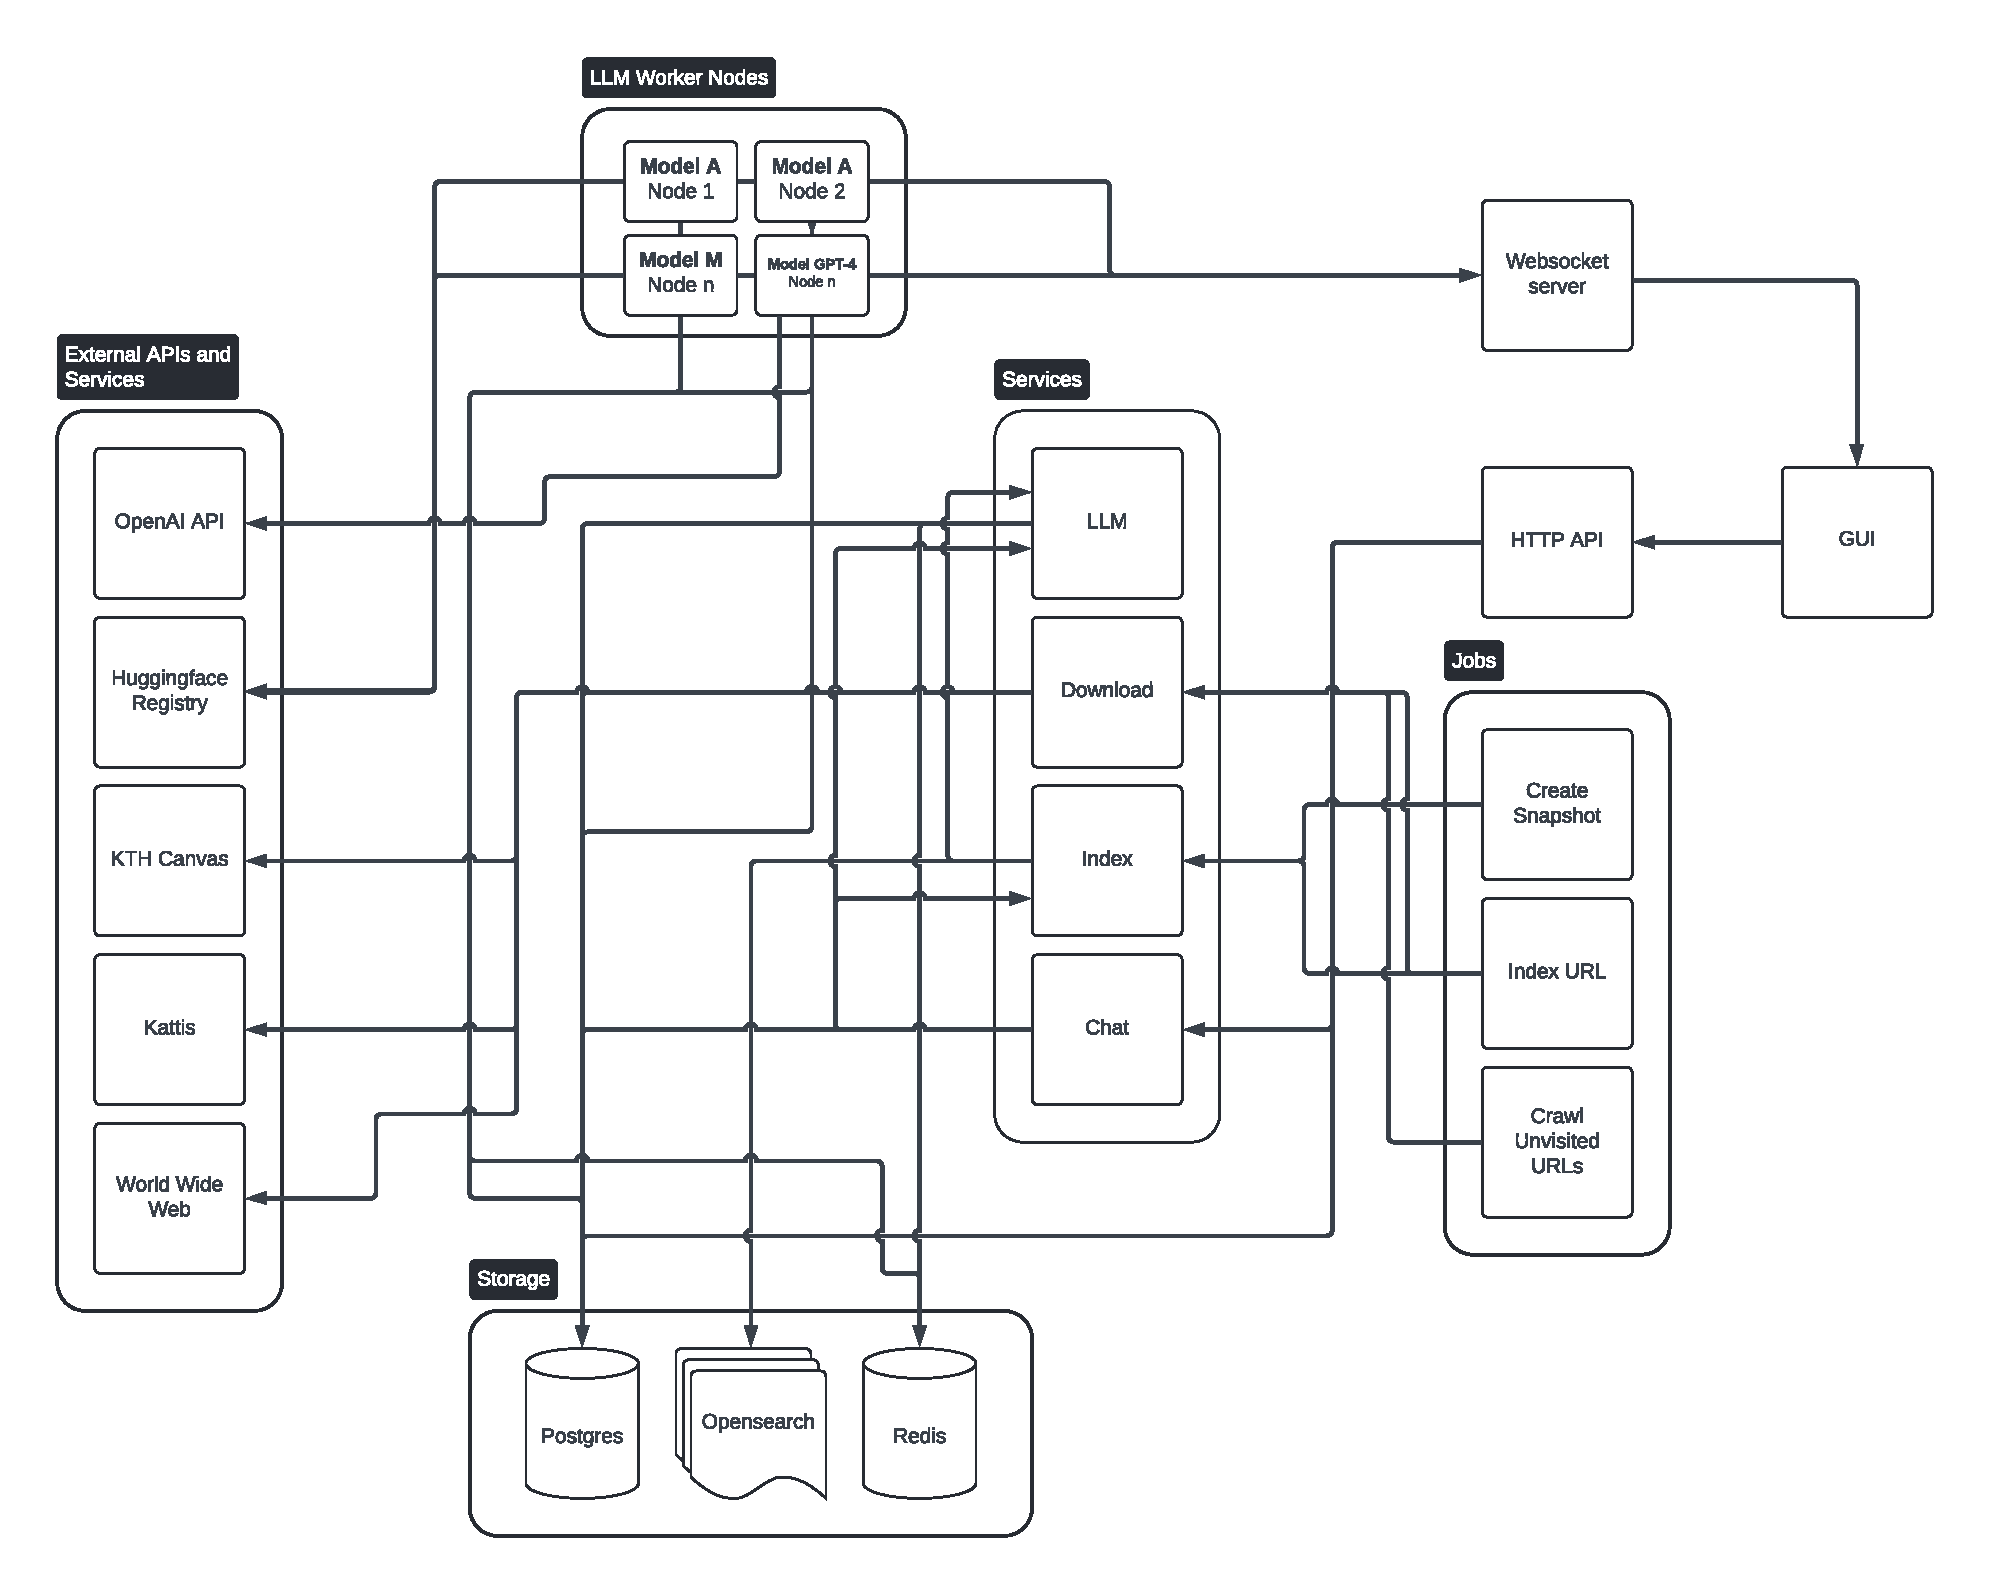
\includegraphics[width=\textwidth]{content/figures/assets/06-system-architecture-diagram.pdf}
    \caption{Diagram that shows the system architecture of the software constructed to run the study}
    \label{fig:system_architecture_diagram}
\end{figure}



\subsection{Courseroom Crawler}


\subsection{Running large language models at scale}


\subsection{Datastore and Index}


\subsection{User interface}


\section{How the software is deployed}


% https://lucid.app/lucidchart/4fca3d7e-5905-40a3-8926-917ce384926b/edit

\begin{figure}[H]
    \centering
    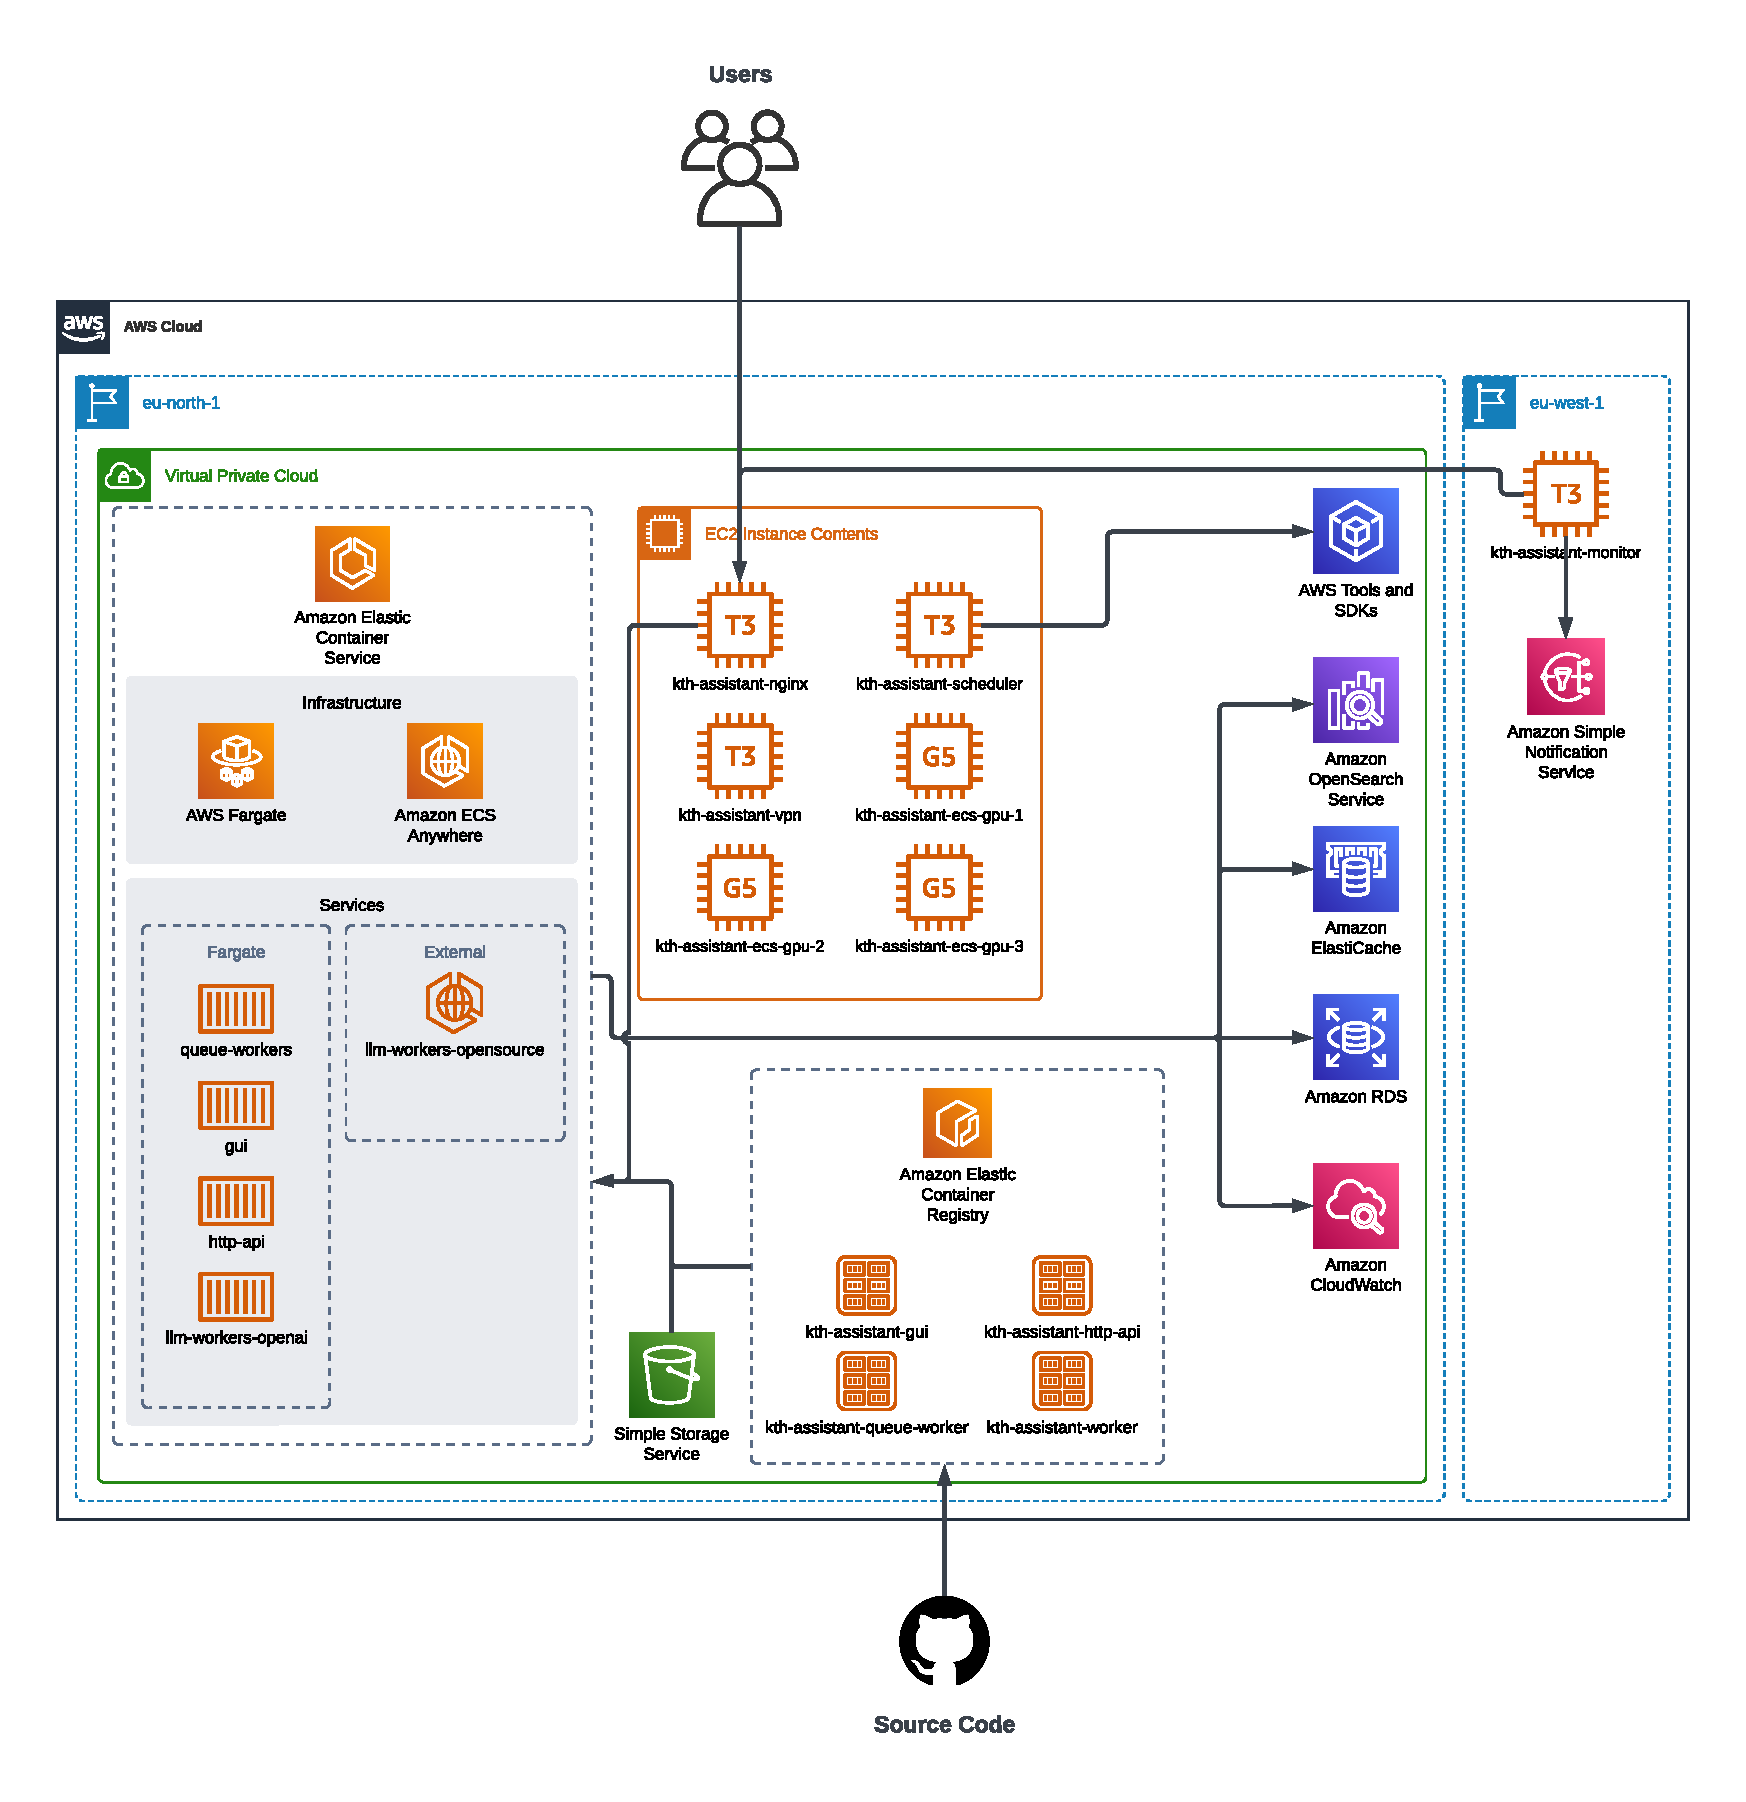
\includegraphics[width=\textwidth]{content/figures/assets/07-aws-diagram.pdf}
    \caption{Diagram that shows how the software was deployed on Amazon AWS}
    \label{fig:aws_diagram}
\end{figure}



% \sweExpl{Hårdvara / Mjukvarudesign ... / modell / Simuleringsmodell och parametrar / …}




% \sweExpl{Figur~\ref{fig:homepageicon}  visar en enkel ikon för en hemsida. Tiden för att få tillgång till den här sidan när den laddas kommer att kvantifieras i en serie experiment. De konfigurationer som har testats i provbänk listas ini tabell~\ref{tab:configstested}.\\
% Vad du har gjort? Hur gjorde du det? Vilka designval gjorde du?}


\section{Implementation …/Modeling/Simulation/…}
\label{sec:implementationDetails}


\subsection{Some examples of coding}


% \engExpl{This section is simply to show some example of how you can include code in your thesis - this is not a section you would have in your thesis.}
% \sweExpl{Det här avsnittet är helt enkelt för att visa ett exempel på hur du kan inkludera kod i ditt examensarbete - det här är inte ett avsnitt du skulle ha i ditt examensarbete.}


\subsection{Some examples of figures in tikz}


% \engExpl{This section is simply to show some example of how you can draw your own figures for in your thesis - this is not a section you would have in your thesis.}
% \sweExpl{Det här avsnittet är helt enkelt för att visa ett exempel på hur du kan rita dina egna figurer i ditt examensarbete – det här är inte ett avsnitt du skulle ha i ditt examensarbete.}
% These figures are just some examples to show that you can draw your own figures for in your thesis. This has two advantages: \first you do not have to worry about copyrights -- as these are your own figures and \Second the text is now readable and not simply a picture of text -- so screen readers can read the figure's contents to someone who is listening to the contents of your thesis.


\subsubsection{Azure's Form Recognizer}


\cleardoublepage